%----------------------------------------------------------------------------------------
%	PACKAGES AND OTHER DOCUMENT CONFIGURATIONS
%----------------------------------------------------------------------------------------

\documentclass{article}

\usepackage{fancyhdr} % Required for custom headers
\usepackage{lastpage} % Required to determine the last page for the footer
\usepackage{extramarks} % Required for headers and footers
\usepackage{graphicx} % Required to insert images
\usepackage{pdflscape} % Allow us to make certain pages in landscape orientation
\usepackage{amsmath} % Allow multiple line equations
\usepackage{amssymb}
\usepackage{scrextend}
\usepackage{xcolor}
\usepackage{listings}

\definecolor{mGreen}{rgb}{0,0.6,0}
\definecolor{mGray}{rgb}{0.5,0.5,0.5}
\definecolor{mPurple}{rgb}{0.58,0,0.82}
\definecolor{backgroundColour}{rgb}{0.95,0.95,0.92}

\lstdefinestyle{CStyle}{
    backgroundcolor=\color{backgroundColour},   
    commentstyle=\color{mGreen},
    keywordstyle=\color{magenta},
    numberstyle=\tiny\color{mGray},
    stringstyle=\color{mPurple},
    basicstyle=\footnotesize,
    breakatwhitespace=false,         
    breaklines=true,                 
    captionpos=b,                    
    keepspaces=true,                 
    numbers=none,                   
    numbersep=5pt,                  
    showspaces=false,                
    showstringspaces=false,
    showtabs=false,                  
    tabsize=2,
    language=C
}

\lstdefinestyle{CStyleInline}{
    backgroundcolor=\color{white},   
    commentstyle=\color{mGreen},
    keywordstyle=\color{magenta},
    numberstyle=\tiny\color{mGray},
    stringstyle=\color{mPurple},
    basicstyle=\footnotesize,
    breakatwhitespace=false,         
    breaklines=true,                 
    captionpos=b,                    
    keepspaces=true,                 
    numbers=none,                   
    numbersep=5pt,                  
    showspaces=false,                
    showstringspaces=false,
    showtabs=false,                  
    tabsize=2,
    language=C
}

% Margins
\topmargin=-0.45in
\evensidemargin=0in
\oddsidemargin=0in
\textwidth=6.5in
\textheight=9.0in
\headsep=0.25in 

\linespread{1.1} % Line spacing

% Set up the header and footer
\pagestyle{fancy}
\chead{} % Top center header
\lhead{\Title}
\rhead{Pedro Alves (9424342)} % Top right header
\lfoot{} % Bottom left footer
\cfoot{} % Bottom center footer
\rfoot{Page\ \thepage\ of\ \pageref{LastPage}} % Bottom right footer
\renewcommand\headrulewidth{0.4pt} % Size of the header rule
\renewcommand\footrulewidth{0.4pt} % Size of the footer rule

\setlength\parindent{0pt} % Removes all indentation from paragraphs

%----------------------------------------------------------------------------------------
%	DOCUMENT STRUCTURE COMMANDS
%----------------------------------------------------------------------------------------

\setcounter{secnumdepth}{0} % Removes default section numbers
   
%----------------------------------------------------------------------------------------
%	NAME AND CLASS SECTION
%----------------------------------------------------------------------------------------

\newcommand{\Title}{Assignment 2} % Assignment title
\newcommand{\DueDate}{21 April 2018} % Due date
\newcommand{\Class}{CAB202 - Microprocessors and Digital Systems} % Course/class
\newcommand{\AuthorName}{Pedro Alves (n9424342)}

%----------------------------------------------------------------------------------------
%	TITLE PAGE
%----------------------------------------------------------------------------------------

\title{
\vspace{2in}
\textmd{\huge\textbf{\Class}}\\
\textmd{{\Title}}\\
\vspace{3in}
\textmd{{\AuthorName}}\\
}

%----------------------------------------------------------------------------------------

\begin{document}

\maketitle
\clearpage

%----------------------------------------------------------------------------------------
%	EXECUTIVE SUMMARY
%----------------------------------------------------------------------------------------
\section*{Executive Summary}

\clearpage

%----------------------------------------------------------------------------------------
%	TABLE OF CONTENTS
%----------------------------------------------------------------------------------------

%\setcounter{tocdepth}{1} % Uncomment this line if you don't want subsections listed in the ToC

\newpage
\tableofcontents
\newpage

%----------------------------------------------------------------------------------------
%	INSTRUCTIONS
%----------------------------------------------------------------------------------------
\section{Instructions}
\begin{enumerate}
	\item Attempt to drive as far as possible without running out of fuel or HP. You win by crossing the finish line
	\item HP is lost by hitting obstacles
	\item Immediate death if a fuel station is hit
	\item To refuel, hold break while immediately next to a fuel station. The car will be pitted automatically if travelling under the pit limit (speed less than 3) with the breaks held
\end{enumerate}
\subsection*{General}
\begin{center}
\begin{tabular}{ c c c }
Function 	& Input 		& Key \\ \hline
Decrease contrast	& Scroll right up 	& Pot1	\\
Increase constrast 	& Scroll right down	& Pot1	\\
\end{tabular}
\end{center}

\subsection*{Splash Screen}
\begin{center}
\begin{tabular}{ c c c }
 Function 	& Input 		& Key \\ \hline
 Play game 	& Left button 	& SW2 \\  
 Play gmae 	& Right button 	& SW3    
\end{tabular}
\end{center}

\subsection*{Game}
\begin{center}
\begin{tabular}{ c c c }
 Function 	& Input 		& Key \\ \hline
 Move left	& Joystick left	& SW1	\\
 Move right	& Joystick right	& SW1	\\
 Pause	& Joystick center 	& SW1	\\
 Accelerate	& Button right	& SW3	\\ 
 Decelerate	& Button left		& SW2	\\
 Limit speed	&			&		\\
 Increase Limit & Left scroll up 	& Pot0	\\
 Decrease Limit & Left scroll down & Pot0
\end{tabular}
\end{center}

\subsection*{Game Paused}
\begin{center}
\begin{tabular}{ c c c }
Function 	& Input 		& Key \\ \hline
Unpause	& Joystick center 	& SW1	\\
Save game	& Joystick up 	& SW1	\\
Load game 	& Joystick down	& SW1	\\
\end{tabular}
\end{center}

\subsection*{Game Over screen}
\begin{center}
\begin{tabular}{ c c c }
Function 	& Input 		& Key \\ \hline
Play again	& Button right	& SW3	\\
Splash screen& Button left 	& SW2 	\\
Load game 	& Joystick down 	& SW1	\\
\end{tabular}
\end{center}

\clearpage

%----------------------------------------------------------------------------------------
%	PROGRAM OVERVIEW
%----------------------------------------------------------------------------------------
\section{Program Overview}
\emph{Zombie Race} is a top-down racing game where the player attempts to drive as far as possible without running out of fuel or colliding with an obstacle. The implementation of this game has been split into several stages that are explained in the later sections. 
\newline
\newline
The basic architecture of the program is that of a state machine. The states for this program are the different screens which the user can see and each provides different functionalities that will be further explored in their specific sections. 
\begin{lstlisting}[style=CStyle]
	// Lines 
	enum GameScreens {
		START_SCREEN,
		GAME_SCREEN,
		GAMEOVER_SCREEN,
	} game_screen;
\end{lstlisting}
After initial setup is complete, the program enters an infinite loop that runs at a rate of about 60 times per second. Inside the loop are two functions, \emph{update()} and \emph{draw()}.
\begin{lstlisting}[style=CStyle]
	// Lines 
	void update(void)
\end{lstlisting}
This function calls the specific update function for the current state the game is in. It will also handle input from \emph{Pot0} that controls the current contrast level of the LCD screen and will perform some operations to allow other functions to use edge detection of the teensy's inputs (ie. only update when clicked). 
\begin{lstlisting}[style=CStyle]
	// Lines 
	void draw(void)
\end{lstlisting}
Will call the draw function of the current state the program is in. Draw function do not change any variables and serve only to write to the LCD through the use of a buffer or directly. Direct draw calls to the LCD will be further explored in the section \emph{Direct screen update}. 
\begin{lstlisting}[style=CStyle]
	// Lines 
	void teensy_setup(void)
\end{lstlisting}
Performs all preliminary calls to setup registers and variables that will be used throughout the program. Will set the clock speed to 8 MHz and the initial LCD contrast to default. The other calls that occur in this functions will be explored in the later sections as they become relevant. 
\clearpage

%----------------------------------------------------------------------------------------
%	TESTING PROCEDURES
%----------------------------------------------------------------------------------------
\section{Testing Procedures}
Due to difficulties with capturing the state of the game directly from the screen of the Teensy, a USB bi-directional communication was set-up between the Teensy and a server. The current value of variables can then be sent as messages to the server in order to assist with debugging, testing and saving/loading. 
\newline
\newline
In order to run the server, enter the command through the Cygwin terminal: \emph{./server /dev/ttyS2} where \emph{ttyS2} is the device name of the Teensy. If this doesn't match, use the command \emph{ls /dev} to find the name for the Teensy currently connected. 
\newline
\newline
The functions used to achieve USB communications will be explored in the section \emph{Bidirectional serial communication and access to file system}. 
\newline
\newline
Testing was accomplished by sending the current state of selected variables via the function \emph{usb\_send\_message()}. Multiple states were then compared to verify if the actual outcome matches the expected outcome.
\newline
\newline
Figure \ref{test_debug} shows the result in the server program when the following command is run
\begin{lstlisting}[style=CStyle]
	usb_send_message(DEBUG, 4, buf, 100, "Timestep: %.3f\nCondition: %d\nFuel: %d\nDistance:  %d\n%d\n", elapsed_time(game_timer_counter), condition, fuel, distance, 0);
\end{lstlisting}
\begin{figure}[!ht]
	\begin{center}
	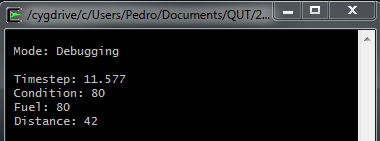
\includegraphics[width=0.8\paperwidth]{images/testing_debug}
	\caption{Screenshot of the server program when a debug command is sent with the current variable states}
	\label{test_debug} 
	\end{center}
\end{figure}
To improve readability of the test plan in the later sections, the information received from the server will be scribed into a table format. Under each teest case, the lines that contain the pieces of code that need to be uncommented to replicate the test are included. 
\clearpage

%----------------------------------------------------------------------------------------
%	SPLASH SCREEN
%----------------------------------------------------------------------------------------
\section{Splash Screen}
The splash screen is the first screen shown when the game is started. After the game is over, the player also has a choice to return to the splash screen. It will display the name of the game and name of the author while waiting for the user to choose to continue playing. The user can choose to start the game by pressing the SW2 or SW3 buttons.

\subsection*{Globals}
\begin{lstlisting}[style=CStyle]
	// Line 
	GameScreens START_SCREEN;
\end{lstlisting}
The value \emph{START\_SCREEN} from the \emph{GameScreens} enum is associated with the splash screen. For more info on the \emph{GameScreens} enum global, see \emph{Program Overview}. 
\begin{lstlisting}[style=CStyle]
	// Line 
	uint8_t button_left_state;
	// Line
	uint8_t button_right_state;
\end{lstlisting}
The current states of the SW2 (left) and SW3 (right) buttons (for more info see \emph{Debouncing}). A state of 1 means the button is pressed. The splash screen will change to the game screen as soon as any of these two variables have a value of 1. 
\newline

\subsection*{Functions}
\begin{lstlisting}[style=CStyle]
	// Lines 
	void start_screen_update(void)
\end{lstlisting}
The update function associated with the splash screen that will be called every tick of the game loop. Will check if SW2 or SW3 have been pressed and call \emph{change\_screen(GAME\_SCREEN)} if true.
\begin{lstlisting}[style=CStyle]
	// Lines 
	void start_screen_draw(void)
\end{lstlisting}
Will call \emph{draw\_string()} to print the name of the game, name of the author and student number to the teensy LCD.  
\newline

\subsection*{Testing}
The following test cases need to pass for this section's tests: 
\begin{itemize}
	\item Game starts when SW2 is pressed
	\item Game starts when SW3 is pressed
\end{itemize}
\subsubsection*{Test Case: Game starts when SW2 or SW3 is pressed}
Lines 457 and 471. A dash in the timestep means that digit was changing rapidly in the server's window.
\begin{center}
\begin{tabular}{ c c c c c }
Timestep	& button\_left\_state	& button\_right\_state	&  game\_screen		& Test result		\\ \hline
0.00-		& 0				& 0				& 1 (START\_SCREEN)	& Pass		\\
0.006		& 0				& 1				& 2 (GAME\_SCREEN)	& Pass		\\
0.00- 		& 0				& 0 				& 1 (START\_SCREEN)	& Pass		\\
0.004		& 1				& 0				& 2 (GAME\_SCREEN)	& Pass		\\ \hline
\end{tabular}
\end{center}
\clearpage

%----------------------------------------------------------------------------------------
%	DASHBOARD
%----------------------------------------------------------------------------------------
\section{Dashboard}
A sub-window in the LCD which displays stats about the player car such as the condition, fuel and speed. A border separates the player from the dashboard area and the player's car is unable to physically move past it (for more info on this, refer to the section \emph{Collision}). It will also display the character 'R' to notify the player that the car is currently refuelling. 

\subsection*{Globals}
\begin{lstlisting}[style=CStyle]
	// Lines 110 - 112
	uint8_t condition;
	uint8_t fuel;
	double speed;
\end{lstlisting}
The variables that hold information about the car. They are modified by other functions thus the dashboard only reads their current values.
\begin{lstlisting}[style=CStyle]
	// Line
	bool refuelling;
\end{lstlisting}
Used to check if the car is currently refuelling. \emph{dashboard\_draw()} will check this and draw the character 'R' if true.
\begin{lstlisting}[style=CStyle]
	// Line
	#define DASHBOARD_BORDER_X  26
\end{lstlisting}
The right-most x coordinate of the dashboard. The border is drawn at this line

\subsection*{Functions}
\begin{lstlisting}[style=CStyle]
	// Lines 
	void dashboard_draw(void);
\end{lstlisting}
Called in the draw function of the game screen. Will draw the line separating the dashboard from the rest of the game screen then will call the \emph{draw\_string()} and \emph{draw\_formatted()} functions in other to display the current game information. If the player is currently refuelling, will display the character 'R' at the bottom. 

\subsection*{Testing}
Testing for this section is a mixture of server and visual analysis. The current values to be displayed on the dashboard are sent to the server and visual analysis of the Teensy's LCD screen will determine if the test has passed.
\subsubsection*{Test Case: Values are correctly displayed}
\begin{center}
\begin{tabular}{ c c c c c }
Timestep	& Condition	& Fuel		& Speed	& Test result	\\ \hline
0.102		& 100		& 100		& 10		& Pass	\\
10.289	& 80		& 78		& 6		& Pass	\\ 
21.383	& 40		& 86		& 1		& Pass	\\ \hline
\end{tabular}
\end{center}

\clearpage

%----------------------------------------------------------------------------------------
%	PAUSED VIEW
%----------------------------------------------------------------------------------------
\section{Paused View}
The user can pause the current game by pressing the center joystick command (SW1). This is only possible when the game state is \emph{GAME\_SCREEN}. The paused screen will display extra information such as the total distance travelled by the car and the elapsed time since the start of the game. While the rest of the game view will be behind the paused view, the player's car can still be visible in order to facilitate the regain of control when unpaused. The time only increases when the game is being played, therefore the counter associated with the current game time must be paused when the paused view is active.

\subsection*{Globals}
\begin{lstlisting}[style=CStyle]
	// Line
	uint8_t distance;
	// Line
	uint16_t game_timer_counter;
\end{lstlisting}
The information that is displayed in the Paused View. These variables are modifed in other sections and Paused View only reads their current value.
\begin{lstlisting}[style=CStyle]
	// Line
	uint8_t game_paused;
\end{lstlisting}

\begin{lstlisting}[style=CStyle]
	// Line
	double time_paused;
\end{lstlisting}

\begin{lstlisting}[style=CStyle]
	// Line
	uint8_t stick_centre_state;
	uint8_t prev_stick_centre_state;
\end{lstlisting}

\clearpage

%----------------------------------------------------------------------------------------
%	CONCLUSION
%----------------------------------------------------------------------------------------
\section{Conclusion}

\end{document}
